\documentclass[11pt,reqno,twoside]{article}
\usepackage[spanish]{babel}

%>>>>>>> RENAME CURRENT FILE TO MATCH LECTURE NUMBER
% E.g., "lecture_01.tex"

%>>>>>>> DO NOT EDIT MACRO FILE

% >>>> DO NOT EDIT THIS FILE
% If you *must* add or change a macro, please email fkoh@caltech.edu

%=================================================
% Basics
%=================================================

\usepackage{fixltx2e} % Makes \( \) equation style robust, among other
                      % things. Must be the first package.


% Makes ligatured fonts searchable and copyable in pdf readers
\usepackage{cmap} % Load before fontenc
\usepackage[spanish]{babel}

% Always include these font encodings in your document
% unless you have a very good reason.
\usepackage[T1]{fontenc}
\usepackage[utf8]{inputenc}

\usepackage{verbatim}

%=====================================
% Look & feel
%=====================================

% Allows for manual space setting
\usepackage{setspace}

%=============
% Fonts
%=============

\usepackage{lmodern} % Improved version of computer modern
\usepackage[scale=0.88]{tgheros} % Helvetica clone for sans serif font


\newcommand\hmmax{2} % Default is 3.
\newcommand\bmmax{2} % Default is 4.

\usepackage{bm} % boldmath must be called after the package
\providecommand{\mathbold}[1]{\bm{#1}}
\usepackage{dsfont}
%=============
% AMS Packages and fonts
%=============
\usepackage{amsmath,amsbsy,amsgen,amscd,amsthm,amsfonts,amssymb}

%=============
% Margins and paper size
%=============
\usepackage[centering,top=1.5in,bottom=1.2in,left=1.4in,right=1.4in]{geometry}

%=============
% Title setup
%=============
\usepackage{titling}
%\usepackage{nopageno}
\setlength{\droptitle}{-7.5em}

\pretitle{\noindent\rule{0.85\linewidth}{0.2mm}\par%
  \begin{raggedright}\LARGE\sffamily}
\posttitle{\par\end{raggedright}%
\noindent%
\rule{0.85\linewidth}{0.5mm}\par}

\preauthor{\noindent\vspace{0.5em}%
  \sffamily\begin{tabular}[t]{ll}}
  \postauthor{\end{tabular}\par\thispagestyle{plain}}

\predate{\noindent%
  \small\sffamily\itshape\begin{tabular}[t]{l}%
    EST-25134, Primavera 2021 \\ %
    Dr.\ Alfredo Garbuno Iñigo \\ %
  }
  \postdate{
  \end{tabular}\par}

%=============
% Section headings
%=============
\usepackage[sf,bf,compact]{titlesec}

%=============
% Tables and lists
%=============
\usepackage{booktabs,longtable,tabu} % Nice tables
\setlength{\tabulinesep}{1mm}
\usepackage[font=small,margin=10pt,labelfont={sf,bf},labelsep={space}]{caption}


\usepackage{enumitem}
\setitemize{itemsep=0pt}
\setenumerate{itemsep=0pt}
\setlist{labelindent=\parindent,%  % Recommended by enumitem package
  font=\sffamily}


%=============
% Hyperlink colors
%=============
\usepackage[usenames,dvipsnames]{xcolor}
\definecolor{dark-gray}{gray}{0.3}
\definecolor{dkgray}{rgb}{.4,.4,.4}
\definecolor{dkblue}{rgb}{0,0,.5}
\definecolor{medblue}{rgb}{0,0,.75}
\definecolor{rust}{rgb}{0.5,0.1,0.1}

\usepackage{url}
\usepackage[colorlinks=true]{hyperref}
\hypersetup{linkcolor=dkblue}
\hypersetup{citecolor=rust}
\hypersetup{urlcolor=rust}
\usepackage[spanish, capitalise]{cleveref}
\usepackage{autonum}
%=============
% Microtype
%=============
\usepackage[final]{microtype}

%=============
% Theorems, etc.
%=============
\newtheoremstyle{myThm} % name
    {\topsep}                    % Space above
    {\topsep}                    % Space below
    {\itshape}                   % Body font
    {}                           % Indent amount
    {\sffamily\bfseries}                   % Theorem head font
    {.}                          % Punctuation after theorem head
    {.5em}                       % Space after theorem head
    {}  % Theorem head spec (can be left empty, meaning ‘normal’)

\newtheoremstyle{myRem} % name
    {\topsep}                    % Space above
    {\topsep}                    % Space below
    {}                   % Body font
    {}                           % Indent amount
    {\sffamily}                   % Theorem head font
    {.}                          % Punctuation after theorem head
    {.5em}                       % Space after theorem head
    {}  % Theorem head spec (can be left empty, meaning ‘normal’)

\newtheoremstyle{myDef} % name
    {\topsep}                    % Space above
    {\topsep}                    % Space below
    {}                   % Body font
    {}                           % Indent amount
    {\sffamily\bfseries}                   % Theorem head font
    {.}                          % Punctuation after theorem head
    {.5em}                       % Space after theorem head
    {}  % Theorem head spec (can be left empty, meaning ‘normal’)

\theoremstyle{myThm}
\newtheorem{theorem}{Teorema}[section]
\newtheorem{lemma}[theorem]{Lemma}
\newtheorem{proposition}[theorem]{Proposition}
\newtheorem{corollary}[theorem]{Corollary}
\newtheorem{fact}[theorem]{Fact}

\theoremstyle{myRem}
\newtheorem{remark}[theorem]{Remark}

\theoremstyle{myDef}
\newtheorem{definition}[theorem]{Definition}
\newtheorem{example}[theorem]{Example}

%=====================
% Header
%=====================
\usepackage{fancyhdr}
\usepackage{nopageno} % Gets rid of page number at the bottom
\fancyhf{} % Clear header style
\renewcommand{\headrulewidth}{0.5pt} % remove the header rule
\pagestyle{fancy}
\fancyhead[LE,RO]{\textsf{\small \thepage}}

\setlength{\headheight}{14pt}
%=====================
% Fix delimiters
%=====================

% Fixes \left and \right spacing issues. See discussion at
% http://tex.stackexchange.com/questions/2607/spacing-around-left-and-right
\let\originalleft\left
\let\originalright\right
\renewcommand{\left}{\mathopen{}\mathclose\bgroup\originalleft}
\renewcommand{\right}{\aftergroup\egroup\originalright}

%=================================================
% Math macros
%=================================================

%=============
% Generalities
%=============
\usepackage{mathtools}
\mathtoolsset{centercolon}  % Makes := typeset correctly for definitions

%%% Equation numbering
%\numberwithin{equation}{section}

%%% Annotations
\newcommand{\notate}[1]{\textcolor{red}{\textbf{[#1]}}}

%==============
% Symbols
%==============
\let\oldphi\phi
\let\oldeps\epsilon
\let\oldemptyset\emptyset
\let\emptyset\varnothing

\renewcommand{\phi}{\varphi}
\renewcommand{\epsilon}{\varepsilon}
\newcommand{\eps}{\varepsilon}
\newcommand{\cl}{\mathrm{cl}}
\newcommand{\wto}{\rightharpoonup}
\newcommand{\wsto}{\overset{\ast}{\rightharpoonup}}
\newcommand{\wwto}{\overset{w}{\to}}
\newcommand{\wwsto}{\overset{w*}{\to}}

%==============
% Constants
%==============

% Set constants upright
\newcommand{\cnst}[1]{\mathrm{#1}}
\newcommand{\econst}{\mathrm{e}}
\newcommand{\rd}{\mathrm{d}}
\newcommand{\dist}{\mathrm{dist}}

\newcommand{\zerovct}{\vct{0}} % Zero vector
\newcommand{\Id}{\mathbf{I}} % Identity matrix
\newcommand{\onemtx}{\bm{1}}
\newcommand{\zeromtx}{\bm{0}}

%==============
% Sets
%==============
\providecommand{\mathbbm}{\mathbb} % In case we don't load bbm

% Reals, complex, naturals, integers, field
\newcommand{\R}{\mathbbm{R}}
\newcommand{\C}{\mathbbm{C}}
\newcommand{\N}{\mathbbm{N}}
\newcommand{\Z}{\mathbbm{Z}}
\newcommand{\F}{\mathbbm{F}}

%==============
% Probability
%==============
\newcommand{\Prob}{\operatorname{\mathbbm{P}}}
\newcommand{\Expect}{\operatorname{\mathbb{E}}}
\newcommand{\D}{\operatorname{\mathcal{D}}}

%==============
% Vectors and matrices
%==============
\newcommand{\vct}[1]{\mathbold{#1}}
\newcommand{\mtx}[1]{\mathbold{#1}}

%=============
% Operators
%=============
\newcommand{\B}{\mathcal{B}}
\newcommand{\op}[1]{\mathbold{#1}}
\renewcommand{\H}{\mathcal{H}}
\newcommand{\X}{\mathcal{X}}
\newcommand{\Y}{\mathcal{Y}}
 % "macro.tex" must be in the same folder

%>>>>>>> IF NEEDED, ADD A NEW FILE WITH YOUR OWN MACROS

% \input{lecture_01_macro.tex} % Name of supplemental macros should match lecture number

%>>>>>>> LECTURE NUMBER AND TITLE
\title{Clase 0:               % UPDATE LECTURE NUMBER
    Aprendizaje Estadístico}	% UPDATE TITLE
% TIP:  Use "\\" to break the title into more than one line.

%>>>>>>> DATE OF LECTURE
\date{Enero 14, 2021} % Hard-code lecture date. Don't use "\today"

%>>>>>>> NAME OF SCRIBE(S)
\author{%
  Responsable:&
  Mr Bean  % >>>>> SCRIBE NAME(S)
}

\begin{document}
\maketitle %  LEAVE HERE
% The command above causes the title to be displayed.

%>>>>> DELETE ALL CONTENT UNTIL "\end{document}"
% This is the body of your document.

\section{Introduction}
\label{sec:introduction}

This document will help you get started writing up the lecture notes. Remember, these notes will be used by you and your classmates, so please work to make them clear and concise.  Below, you will find some rules designed to ensure consistency in the course notes as well as some tips for getting the most from this file.

\subsection{The basics}

In order to typeset this file, you need to have a reasonably up-to-date copy of \LaTeX\ installed on your system.  This free software is available from \url{http://tug.org}.   See Section~\ref{sec:need-help} for information on where to get more help setting up \LaTeX, typesetting math, and other technical issues.

To get started, download and extract the \texttt{template.zip} file from Piazza. This compressed folder contains the following files.
\begin{description}
  \setlength{\itemsep}{0pt} \setlength{\topsep}{0pt} % Make list compact
\item[\texttt{template.pdf}] \emph{This formatted document.}
\item[\texttt{template.tex}] \emph{Contains the source code for this document.} The comments indicate the changes that you need to make to start your document. For example, you  need to add the lecture number and title, include the name(s) of the scribe(s), and hardcode the date of the lecture.
\item[\texttt{template.bib}] \emph{Provides BibTeX references.}
\item[\texttt{macro.tex}] \emph{Defines layout and provides shortcuts.}
\item[\texttt{bell\_curve\_hand.jpg}, \texttt{bell\_curve\_matlab.pdf}]  \emph{The image files for Figure~\ref{fig:bell-curve}.}
\end{description}
To compile this document from a UNIX command line, run the following four commands.
\begin{center}
  \begin{minipage}[c]{0.3\linewidth}
\begin{verbatim}
 pdflatex template.tex
 bibtex template
 pdflatex template.tex
 pdflatex template.tex
\end{verbatim}
  \end{minipage}
\end{center}

\subsection{Setting up your lecture notes}
\label{sec:setting-up-your}

Rename all \texttt{template.*} files to \texttt{lecture\_XX.*}, where \texttt{XX} is the lecture number. For example, the source file for the first lecture will be  named \texttt{lecture\_01.tex}.  If  you need to include references,  include the appropriately formatted BibTeX entries in your \texttt{lecture\_XX.bib} file.  You will submit these files, as well as any figures required to compile the notes.

\section{Rules \& regulations}
\label{sec:rules}
In order to make the notes as consistent as possible, we are going to enforce a few ground rules.  These rules are meant as guides, but whenever common sense and these rules conflict, the former prevails.



\subsection{Style}
\label{sec:style}

The most important part of your notes is, of course, the content. But even the best content will fail to impress in the face of haphazard style and inconsistent notation.

\begin{description}\setlength{\itemsep}{0pt} % Compact description list
\item[Spanish] Use complete, grammatically correct Spanish sentences. Consult dictionaries and style guides for proper spelling and usage. For specific guidelines on mathematical writing, see~\cite{Che:,Hal:70,Hig:98}.
\item[Sections] Use \LaTeX's built-in commands for defining sections, subsections, subsubsections, etc.  Whenever possible, use the  section breaks presented in class and their corresponding  titles.  Use common sense when adding and naming additional sections.
\item[Equations] Only number equations that are referenced later in the text.
Refer to Michael Downes's \href{https://math.mit.edu/~dav/short-math-guide.pdf}{Short Math Guide for \LaTeX} for available equation environments.
\item[Theorems, definitions, etc.] Several environments are available for stating formal mathematical results and theorems. For example, the \texttt{theorem} environment typesets theorems:
  \begin{center}
    \begin{minipage}[c]{0.7\linewidth}
      \begin{theorem}[Fermat, Wiles]\label{thm:FermatWiles}
        For any integer \(n\ge 3\) and all \(a,b,c \in \N\), it holds that \(a^n + b^n \ne c^n\).
      \end{theorem}
      \begin{proof}
        Somewhat too long for this note.
      \end{proof}
    \end{minipage}
  \end{center}
  Other environments include \texttt{lemma}, \texttt{proposition}, \texttt{corollary}, \texttt{fact}, \texttt{remark}, \texttt{definition}, and \texttt{example}.
    \item[Figures] Please include figures when appropriate.  Neatly hand-drawn and scanned figures are acceptable, but you are welcome to use computer-generated figures as well. All figures should have appropriate captions. Since we compile using \texttt{pdflatex}, the files must be one of \texttt{.pdf} (for vector graphics), \texttt{.png} (simple diagrams and raster vectors), or \texttt{.jpg} (for pictures). See Figure~\ref{fig:bell-curve} for an example.
    \begin{figure}[h!]
      \centering
      \includegraphics[width=0.4\columnwidth]{bell_curve_hand.jpg}
      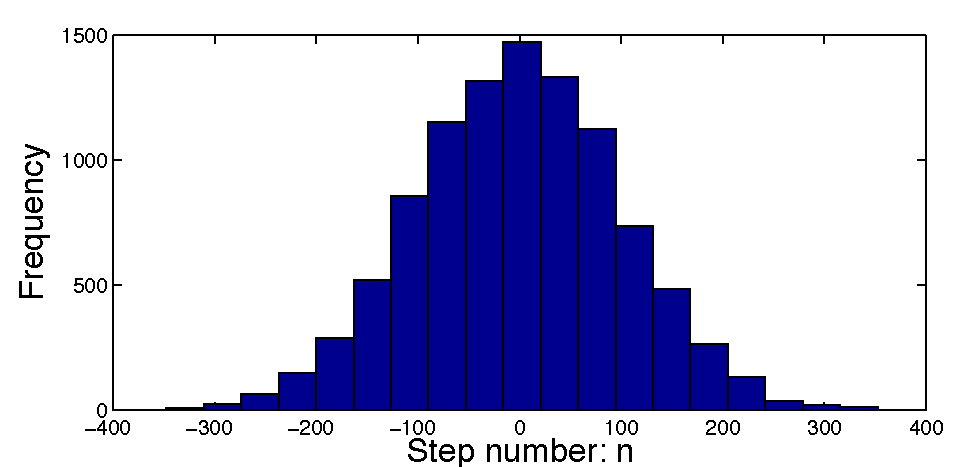
\includegraphics[width=0.55\columnwidth]{bell_curve_matlab.pdf}
      \caption{{\textsf{Example figures.}}  Legible hand-drawn figures [left] are appropriate for the notes, but make sure to adjust the color of scanned images to remove as much gray region as possible.  If you prefer to generate vector-graphics figures [right] using computer software, please adjust the font size so that the labels are legible.  }\label{fig:bell-curve}
    \end{figure}
    \item[Tombstones] Do not let your equations or text extend perceptibly beyond the right margin.  The typesetting system of \LaTeX\ takes care of most tombstones in the text, although on occasion you may need to rephrase a sentence to avoid a dangling word. Equations require more work.  If an equation is too long to fit on a single line, either use the \texttt{multline} or \texttt{align} environments to break long equations into appropriate pieces, or reconsider the way you present the mathematics.
 \item[Punctuation] A mathematical document should follow the standard rules of punctuation, this includes putting commas/periods at the end of equations and mathematical expressions. A good rule of thumb is to place punctuation where you would expect it if the mathematics you write would be read out as words. If a comma/period is at the end of an equation (e.g. in \texttt{equation}, \texttt{align} or \texttt{multiline} environments), it is preceded by \verb|\,| to create a small space. For example, the equation $a^n + b^n \ne c^n$ from Theorem \ref{thm:FermatWiles} on a separate line should be displayed as
  \begin{equation*}
      a^n + b^n \ne c^n \,.
  \end{equation*}
\item[Notation] Stick to the notation used in class whenever possible.  For consistency, we defined the following notation using macros.

    \begin{minipage}[c]{\linewidth}
      \begin{center}
        \begin{tabu}{ccc}
          \toprule
          \textbf{Purpose} &  \textbf{Example} \\
          \midrule
          Naturals, integers  & $\N$, $\Z$
          \\
          Reals, complex  & $\R$, $\C$
          \\
          Fields (reals or complex) & $\F$
          \\
          Norms & $\| \cdot \|$
          \\
          Inner Product & $ \langle \cdot, \cdot \rangle$
          \\
          Expectations & $\Expect_{z \sim \D}[f(z)]$
          \\
          Limits & $\underset{\theta \in \Theta}{\sup} \,\, \mathcal{L}_n(\theta)$
          \\
          \bottomrule
        \end{tabu}
      \end{center}
    \end{minipage}

    Consult the source file \texttt{template.tex} for the commands used to create this table. In addition, we use the convention of a straight $\rd$ for integrals, preceded by \verb|\,| to create a small space, see the command for $\int f(x)\, \rd x$ in the source file.
  \item[Cross-references] Use \LaTeX's built-in facility to label and cross-reference sections, theorems, tables, figures, and equations. For example, this text is in Section~\ref{sec:style}, which begins on Page~\pageref{sec:style}. Hardcoding references makes your document fragile. It also does not take advantage of the PDF hyperlinking provided by the \texttt{hyperref} package.
  \item[Bibliography] If you need to cite an article, use the \texttt{bibtex} program with  bibliography style \texttt{alpha}.  Format the entries according to the AMS style, including the correct \href{http://www.ams.org/msnhtml/serials.pdf}{abbreviations of the names of serials}. For many published mathematics articles, you can download reviewed and correctly formatted \texttt{bibtex} citations from the AMS MathSciNet website~\cite{mathscinet}. Include the BibTeX references in your \texttt{lecture\_XX.bib} file when you submit your work.

\end{description}

\subsection{Editing}
\label{sec:editing}

No written document is complete without a thorough editing, and a number of tools are available to help you edit your \LaTeX\ files.  A quick search on the web turns up several spell-checkers.  Unfortunately, automatic grammar checkers prove  useless for mathematical documents because of the large number of equations. Thus, you must check the grammar by hand.

Several useful tools are available for collaborative editing of \LaTeX\ documents.  We often use the \texttt{\textbackslash notate} macro that \notate{highlights text in red}.  Some utilities included in the  \TeX\ distribution include \texttt{latexdiff}, which shows differences between \TeX\ files, and \textit{Excalibur},  a \LaTeX-aware spell-checker.

\subsection{You have your \emph{own} macros, you say?}
\label{sec:macros}

Our goal is to obtain a consistent set of lecture notes for the benefit of the whole class.  Ideally, we will compile them into a single paginated document with a table of contents.  This is impossible if scribes change the macros or add their own.

To that end, please use the macros that are defined in \texttt{macro.tex}.  Do not redefine these macros.  Do not use \texttt{\textbackslash renewcommand}.  If you must have your own macros, please put them in a separate file named \texttt{lecture\_XX\_macros.tex} where \texttt{XX} is the lecture number.  Make sure there are no collisions with existing macros.


\section{Need help?}
\label{sec:need-help}

For information on typesetting mathematics using \LaTeX, we recommend Michael Downes's \href{https://math.mit.edu/~dav/short-math-guide.pdf}{Short Math Guide for \LaTeX} and the references therein.
Numerous additional resources for \LaTeX\ are available on the web, including the \href{http://tex.stackexchange.com/}{\TeX\ StackExchange} website,
and we encourage you to search for answers to any problems that arise online \emph{before} contacting the instructor or the TA.

If you find an error in the template or macro file, please email a description of the problem, and any fix that you have in mind, to \href{mailto:fkoh@caltech.edu}{fkoh@caltech.edu}.


%>>>>>> END OF YOUR CONTENT

%>>>>>>>>>> take acknowledgements out
\section*{Acknowledgements} This template has been adapted from a lecture note template for ACM 204 (Fall 2017) by Prof Joel Tropp.


\bibliographystyle{alpha} % <<< USE "alpha" BIBLIOGRAPHY STYLE
\bibliography{template} % <<< RENAME TO "lecture_XX"


\end{document}
